\chapter{Réalisations techniques}
Comme énoncé dans la première partie de ce mémoire, nus allons concentrer notre travail sur la sécurisation des 
développements applicatifs jusqu'à leur déploiement. Nous aborderons donc des sujets tel que la création de deux 
procédures de sécurité, l'outillage des équipes ainsi que la réalisation de diverses évaluations de sécurité.

\section{Une première approche du DevSecOps}
Rapidement évoqué dans l'état de l'art, l'équipe de \ac{SSI} a entamée ,dès le quatrième semestre de 2018, un premier 
travail d'intégration de sécurité informatique dans les développements au travers de la mise en place d'un processus 
\emph{Security By Design}.

Ce processus, centré en son cœur sur l'accompagnement de \emph{Security Champions}\footnote{Un 
\emph{Security Champion} est un ambassadeur de la \ac{SSI} dans les équipes projets.}, vise à faciliter le questionnement
et  les réflexions sur les sujets de \ac{SSI} dans les équipes projets. Représentés par des responsables produit, des 
développeurs ou opérationnels, ils favorisent les échanges entre les équipes projets et l'équipe de \ac{SSI} en servant 
de réels points de liaisons pour ces dernières.

Grâce au travail des \emph{Security Champions}, le nombre de demande d'audit technique et de conseils d'architecture
a progressivement augmenté tout au long de l'année 2019. L'équipe s'est donc retrouvé à réaliser plusieurs audits par 
mois sur l'année 2019 là où elle n'en réalisait qu'un tous les deux mois en moyenne en 2018. J'ai par ailleurs eu le 
plaisir de m'occuper d'une majorité de ces qualifications sécurité.

C'est d'ailleurs sur cette même période qu'un projet de personnalisations des règles du \ac{SAST} (SonarQube) exploité 
par JCDecaux a été lancé. Ces personnalisations, réalisées en deux temps, visaient à créer plusieurs profils d'analyse 
pour chaque langage de programmation utilisé dans l'entreprise, tout en réduisant le bruit généré par des règles 
remontant trop de faux positif.

Grace à ces actions, portés tant auprès du Groupe qu'auprès de ses filiales, l'équipe de \ac{SSI} s'est rapproché un peu
plus de son objectif de sécurisation des applications développées en interne. Cette approche proactive et non plus 
réactive de sécurisation a notamment permis de réduire drastiquement le nombre d'applications rejetées à la suite d'une 
qualifications sécurité pré-déploiement en production.

Nous passions donc d'une méthodologie agile \emph{DevOps} à une méthodologie \emph{DevSecOps}.

\newpage

\section{Les audits : quel processus pour quel résultat}
Depuis 2019, nous (l'équipe de \ac{SSI}) avons observé une nette augmentation du nombre de qualification sécurité réalisées
aux profits des projets de développement. Cette augmentation, bien que bénéfique à l'objet de l'équipe, a eu pour effet 
de mettre en évidence divers problèmes ans l'organisation et la réalisation de ces audits.
\newline Il nous arrivait encore à cette période de devoir intérrompre la publication de certaines applications n'étant 
pas qualifiées, faute de procédures explicites et partagées à toutes les équipes de JCDecaux. Nous avons donc commencer à 
travailler sur la question avec l'aide de quelques équipes de la \ac{DSI} France.

La première réalisation dans cette quête de structure à été la définition claire et précise des points de contrôle et 
des vulnérabilités recherchées sur les applications. Ces points de contrôle sont fortement inspirés par l'OWASP Top ten
\autocite{owasp_top10_2017} et sont formulés dans un tableur servant à faire leur suivi durant l'audit. Chacun est 
ensuite associé à plusieurs états (testé ou non, risque et application de correctifs) ainsi qu'un commentaire le cas 
échéant.

A cette liste de points de contrôle est ensuite adossé une revue du projet sur SonarQube (note \ac{SAST}) et de la 
classification des entrés remontées par l'outil. Cette étape nous permets de prendre la mesure de la qualité du code de 
l'application audité mais aussi du niveau d'attention apporté par l'équipe de développement à son application.
\newline Nous avons en effet constaté que les projets ayant le plus de vulnérabilité et erreur de code remonté par 
SonarQube étaient géré par des équipe ayant peu d'intérêt dans le contrôle qualité de leur code.
\newline Ce même type de revue est réalisé le niveau de vulnérabilité des conteneurs pour les applications concernées, 
mais nous reviendrons sur ce sujet plus tard.

Nous avons par la suite commencé à travailler sur la définition des livrables et des points abordés durant la réunion de
restitution. Il est important de noté que ces livrables se limitaient jusque là à une simple liste de vulnérabilités
ordonnées en fonction de leur criticité et sans démonstration ou explication du chemin d'attaque.
\newline  La mise en place d'une restitution appropriée et argumentée de l'audit à permis de déceler quelques 
méconnaissance dans plusieurs équipes (notamment vis-à-vis du framework IAM du groupe) et sert souvent de point de départ 
à l'accompagnement des équipes entament leurs migration vers le DevSecOps.

Voilà donc comment fonctionnaient le processus d'audit applicatif entre 2019 et 2020. 
\newline Cependant, ce processus étant tacite et non formaliser (la culture de l'orale étant encore très fort chez 
JCDecaux), plusieurs départs et changements de postes l'on mis à mal.

C'est pourquoi nous avons entrepris de formuler ce processus dans un langage commun (ici le \ac{BPMN}) afin de le partager
aux équipes impliqué dans celui-ci. Nous en avons profité pour intégrer quelques prérequis facilitant l'organisation 
de l'audit technique et la création de garde-fous.

\newpage

Le processus d'audit est donc représenté sous la forme de deux diagrammes : le premier décrivant le fonctionnement 
générale de l'audit et des différent échanges entre l'équipe de développement et l'équipe de \ac{SSI}; le second 
décrivant les actions techniques réalisées durant l'audit.

\begin{figure}[h]
    \centering
    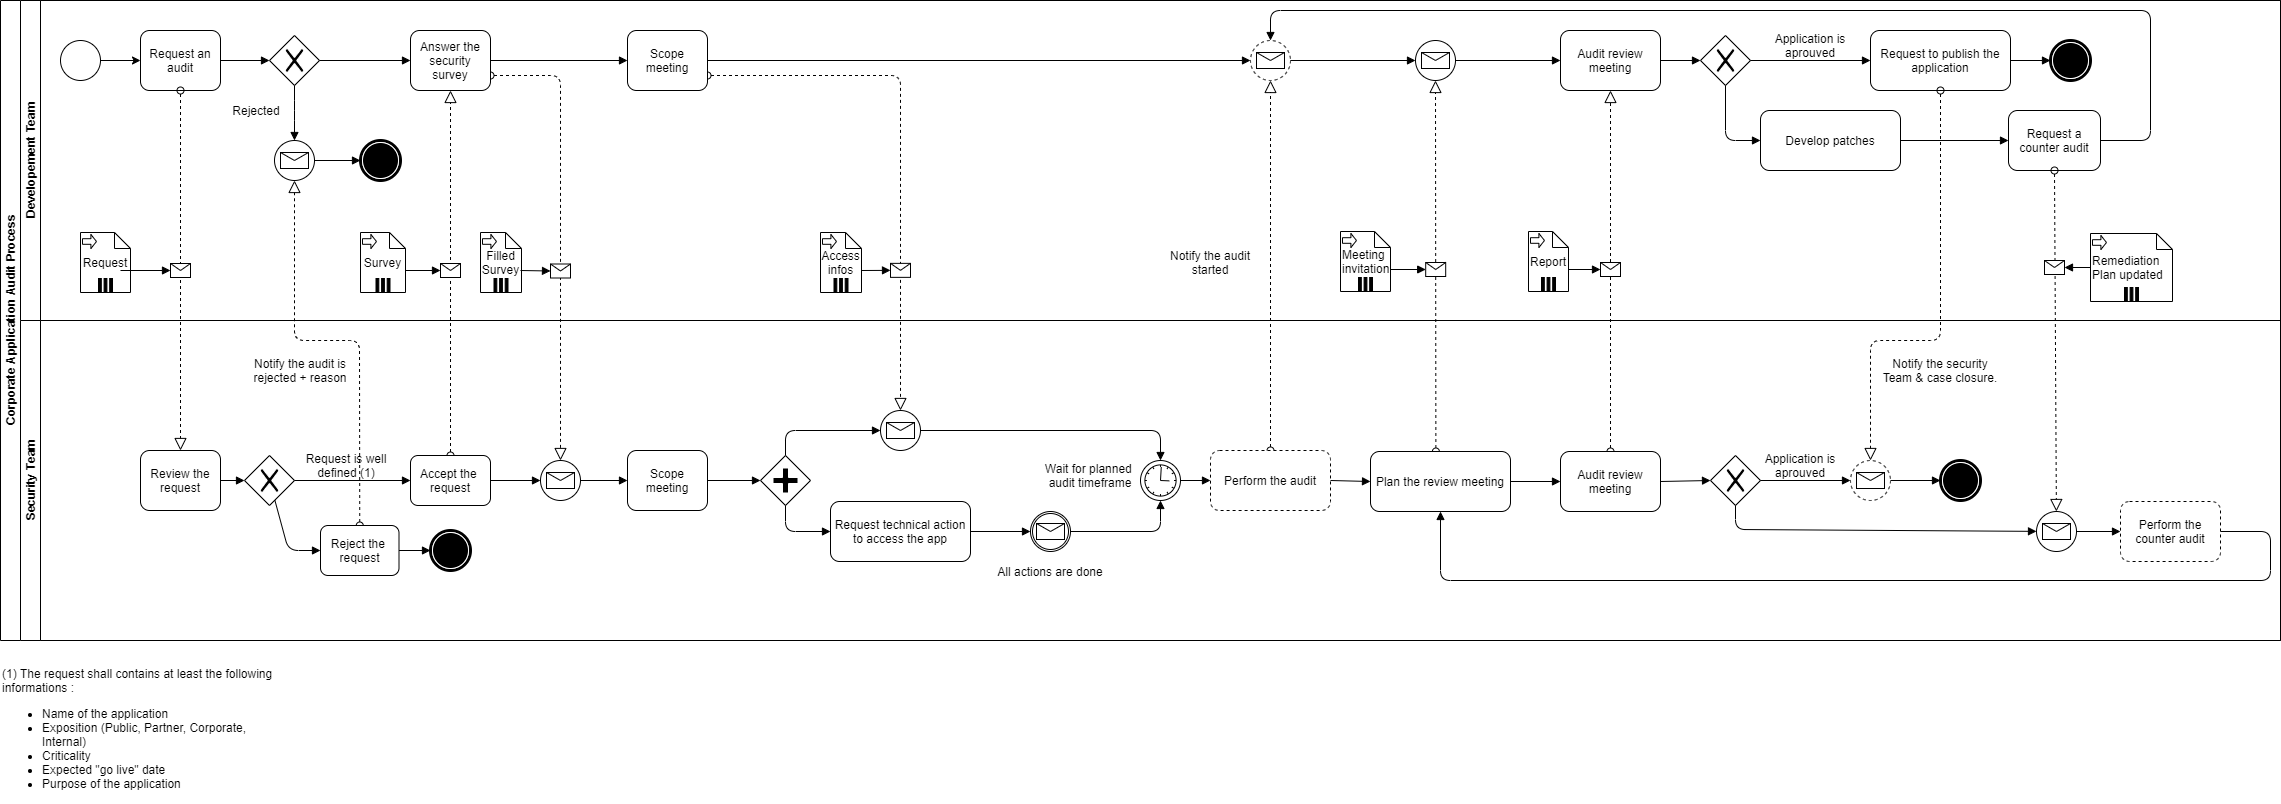
\includegraphics[width=\linewidth]{resources/img/process_audit.png}
    \caption{Processus de l'audit de sécurité d'une application}
\end{figure}

\begin{figure}[h]
    \centering
    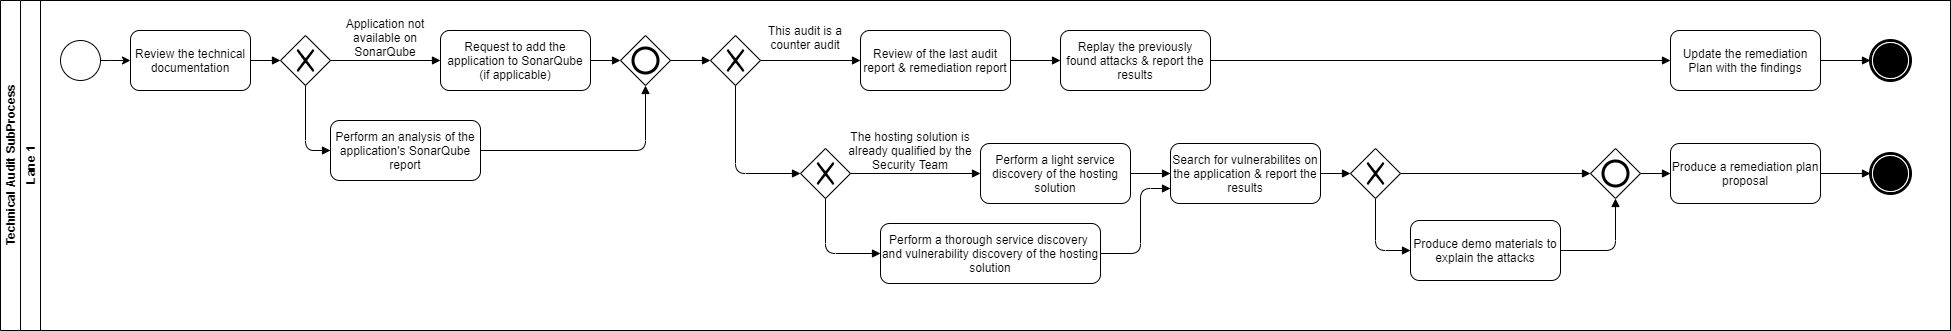
\includegraphics[width=\linewidth]{resources/img/technical_audit_subprocess.png}
    \caption{Processus fils de l'audit de sécurité d'une application : actions techniques}
\end{figure}
\begin{center}
    \colorbox{gray!15}{Ces deux diagrammes étant relativement complexes, vous les retrouverez en annexes}
\end{center}

Nous trouvons donc dans ce processus nouvellement formalisé l'ensemble des éléments précédemment évoqués avec l'ajouts 
de quelques nouveautés nous permettant de mieux préparer l'audit. C'est ainsi qu'est intégrer un questionnaire visant à
fournir à l'équipe de \ac{SSI} des informations supplémentaire sur la nature de l'application devant être audité ainsi 
que les éventuelles contraintes temporelles.

Ce processus étant en place dans sa version finale depuis Avril 2021, nous observons une amélioration progression des 
conditions d'organisation des audits techniques, notamment sur les éléments de contexte relatif aux applications devant 
être audités.
Il s'agissait en effet d'un certain point de friction de septembre 2020 suite au départ d'une de nos collaboratrices.

\newpage

